\cotefile{10}
\scanpage{33}
\mspage{\handwritten{1}}
% archive sheet number: 32

\uline{10. Passage to the projective limit in group preschemes and preschemes with a group of operators.}

\margin{\handwritten{\figure{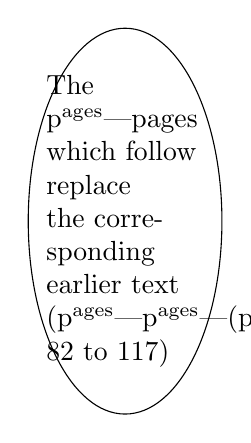
\begin{tikzpicture}
\node[text width=2cm,align=left,inner sep=2pt] at (0,0) {The \unsure{p\textsuperscript{ages}|pages} which follow replace the corresponding earlier text \unsure{(p\textsuperscript{ages}|p\textsuperscript{ages}|(pages|pages} 82 to 117)};
\draw (0,0) ellipse (1.23 and 2.45);
\end{tikzpicture}}}}
\handwritten{10.}0. Let us recall the essential result of (EGA IV 8.8) : Given the following situation : $S_o$ a qu\handwritten{/}asi-compact and quasi-separated prescheme, $I$ an upward filtering preordered set, $(\handwritten{\unsure{\mathscr{A}|\mathcal{A}}}_i)_{i\handwritten{\in}I}$ an inductive system of quasi-coherent commutative $\handwritten{\mathcal{O}}_{S_o}$-Algebras, $\handwritten{\mathscr{A}}=\underset{\handwritten{\longrightarrow}}{\lim}\handwritten{\mathscr{A}}_i$, $S_i=\operatorname{Spec}\handwritten{\mathscr{A}}_i$ for $i\handwritten{\in}I$, and $S=\operatorname{Spec}\handwritten{\mathscr{A}}$, \handwritten{t}hen the category of $S$-preschemes of finite presentation is determined up to equivalence by the data of the categories of $S_i$-preschemes of finite presentation, of the functors \inserted{between these categories} $\handwritten{\rho}_{ij}:X_i\handwritten{\rightsquigarrow}X_i\times_{S_i}S_j$ \deleted{\unsure{,}} for $i\handwritten{\leqq}j$, and of the transitivity isomorphisms $\handwritten{\rho}_{jk}\mathbin{\unsure{o|\circ}}\handwritten{\rho}_{ij}\handwritten{\xrightarrow{\sim}\rho}_{ik}$. \deleted{More precisely,} \handwritten{Let us be precise.}

\margin{\handwritten{\figure{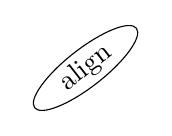
\begin{tikzpicture}
\node[rotate=38,inner sep=1pt] at (0,0) {align};
\draw[rotate=38] (0,0) ellipse (.82 and .24);
\end{tikzpicture}}\quad )\quad )}}
Given $j\handwritten{\in}I$, and an $S_j$-prescheme of finite presentation $X_j$, we shall set,for every $i\handwritten{\in}I$ such that $j\handwritten{\leqq}i$, $X_i=X_j\handwritten{\times}_{S_j}S_i$, and $X=X_j\handwritten{\times}_{S_j}S$. Then :\inserted{\handwritten{(EGA \uline{IV} 8.8.2)}}\handwritten{\unsure{;|:}}\margin{\handwritten{(}}

\uline{i) Given $j\handwritten{\in}I$, and two $S_j$-preschemes of finite presentation $X_j$ and $Y_j$, the canonical map from $\underset{i\handwritten{\geqslant}j}{\underset{\handwritten{\longrightarrow}}{\lim}}\operatorname{Hom} S_i(X_i,Y_i)$ to $\operatorname{Hom}(X,Y)$ is bijective}\margin{\handwritten{(}}

\uline{ii) For every $S$-prescheme of finite presentation $X$, there exists an index $j\handwritten{\in}I$, \deleted{and} an $S_j$-prescheme of finite presentation $X_j$ and an $S$-isomorphism $X\handwritten{\xrightarrow{\sim}}X_j\handwritten{\times}_{S_j}S$.}

One concludes from this (EGA IV 8.8.3) that, whenever one has a diagram $D$ involving a finite number of objects and arrows of the category of $S$-preschemes of finite presentation, one can find an index $i\handwritten{\in}I$ and a diagram $D_i$ in the category of $S_i$-preschemes of finite presentation, such that the diagram $D$ arises up to isomorphism from the diagram $D_i$ by the base change $S\handwritten{\longrightarrow}S_i$. One can even find $i$ and $D_i$ such that every cartesian square of $D$ arises from a cartesian square of $D_i$.

\handwritten{10.1.} Moreover, a large number of properties \deleted{of} usual for a morphism, stable under base change, possess the following property ; given an index $j\handwritten{\in}I$ tw\deleted{s}\inserted{\handwritten{o}} $S_j$-preschemes of finite presentation $X_j$ and $Y_j$ and an $S_j$-morphism $u_j:X_j\handwritten{\longrightarrow}Y_j$, for $u=u_j\handwritten{\times}_{S_j}S$ to have the property $\handwritten{\mathbb{P}}$, it is necessary and sufficient that there exist an index $i\handwritten{\in}I$ such that $j\handwritten{\leqq}i$ and that $u_i=u_j\handwritten{\times}_{S_j}S_i$ have the property $\handwritten{\mathbb{P}}$. This is so in the case where $\handwritten{\mathbb{P}}$ is \deleted{the}\inserted{\handwritten{one of the}} \inserted{\handwritten{following}} propert\inserted{\handwritten{ies}} for a morphism:\deleted{\unsure{of}} being separated, surjective, radicial, affine, quasi-affine, finite, quasi-finite, proper, projective, quasi-projective, an isomor%
